
Being aware of how much of your code is covered by tests is a great benefit and often gives a very good impression about how well-tested a given software is. It can also give hints to developers about the execution paths and edge cases that are not covered by tests.

There are a few tools that help you get code coverage in C++. Arguably, the most popular is Gcov from GNU. It's been around for years and works well with GCC and Clang. Although it does not work with Microsoft's Visual Studio, using Clang to build and run the software provides a viable alternative for Windows. Alternatively, the tool OpenCppCoverage can be used to get coverage data on Windows to build with MSVC.

The coverage information generated by Gcov can be collected in summarized reports with the Gcovr or LCOV tools.

\subsubsubsection{7.3.1\hspace{0.2cm}Generating coverage reports using Clang or GCC}

In this section, we will look at how to create such reports with Gcovr. Generating code coverage reports roughly works in the following way:

\begin{enumerate}
\item 
The program and libraries to be tested are compiled with special flags so they expose the coverage information.

\item 
The program is run and the coverage information is stored in a file.

\item 
The coverage analyzers, such as Gcovr or LCOV, analyze the coverage files and generate reports.

\item 
Optionally, the reports are stored or further analyzed to display trends in coverage.
\end{enumerate}

A common setting for code coverage is that you want to have information about how much of the code of a project is covered by the unit tests. In order to do this, the code has to be compiled with the necessary flags so the information is exposed.

The <LANG>\_COMPILER\_FLAGS cache variable should be passed to CMake over the command line. When using GCC or Clang, this might look like this:

\begin{tcblisting}{commandshell={}}
cmake -S <sourceDir> -B <BuildDir> -DCMAKE_CXX_FLAGS=--coverage
\end{tcblisting}

An alternative is to define the respective preset, as explained in Chapter 9, Creating Reproducible Build Environments. When building for coverage, it is often a good idea to compile with the debug information enabled and to disable any optimization with the -Og flag. Additionally, specifying the -fkeep-inline-functions and -fkeep-staticconsts compiler flags will prevent optimizing away static and inlined functions if they are never used. This will make sure that all possible execution branches are compiled into the code, otherwise, the coverage report might be misleading, especially for inlined functions. 

Coverage reports work not just for single executables, but also for libraries. However, the libraries also have to be compiled with the coverage flags on.

As the compiler flags for coverage are set globally, the options will be passed on to projects added with FetchContent or ExternalProject, which might increase the compile time considerably.

Compiling sources using GCC or Clang with the coverage flag enabled will create .gcno files in the build directories for each object file and executable. These files contain the meta information for Gcov about which calls and execution paths are available in the respective compilation units. In order to find out which of these paths are used, the programs have to be run.

For the setting where we want to find out the code coverage of the tests, running CTestwill generate the coverage results. Alternatively, running the executables directly will produce the same results. Running executables with coverage enabled will generate .gcda files in the build directories that contain the information about the calls in the respective object files.

Once these files are generated, running Gcovr on them will create the information about coverage. By default, Gcovr outputs the information to stdout, but it can also generate HTML pages, JSON files, or SonarQube reports.

\begin{tcblisting}{commandshell={}}
gcovr -r <SOURCE_DIR> <BINARY_DIR> -html
\end{tcblisting}

Such a call might produce an HTML file that looks like this:

\begin{center}
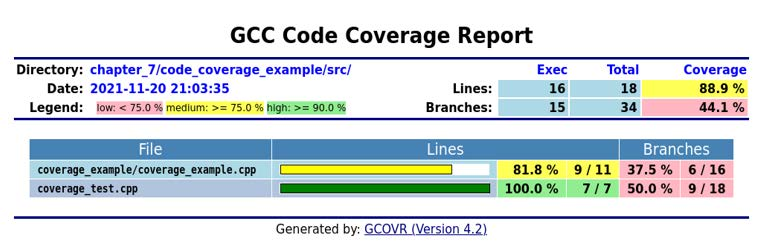
\includegraphics[width=0.8\textwidth]{content/2/chapter7/images/1.jpg}\\
Figure 7.1 – An example output for a coverage run
\end{center}

Another alternative to Gcovr is LCOV, which works in a very similar way. In contrast to Gcovr, LCOV cannot directly produce HTML or XML output but will assemble any coverage information in an intermediate format, which can then be consumed by various converters. To produce HTML output, the genhtml tool is often used. To generate a report using LCOV, the commands could look like this:

\begin{tcblisting}{commandshell={}}
lcov -c -d <BINARY_DIR> -o <OUTPUT_FILE>
genhtml -o <HTML_OUTPUT_PATH> <LCOV_OUTPUT>
\end{tcblisting}

A coverage report generated with LCOV might look like this:

\begin{center}
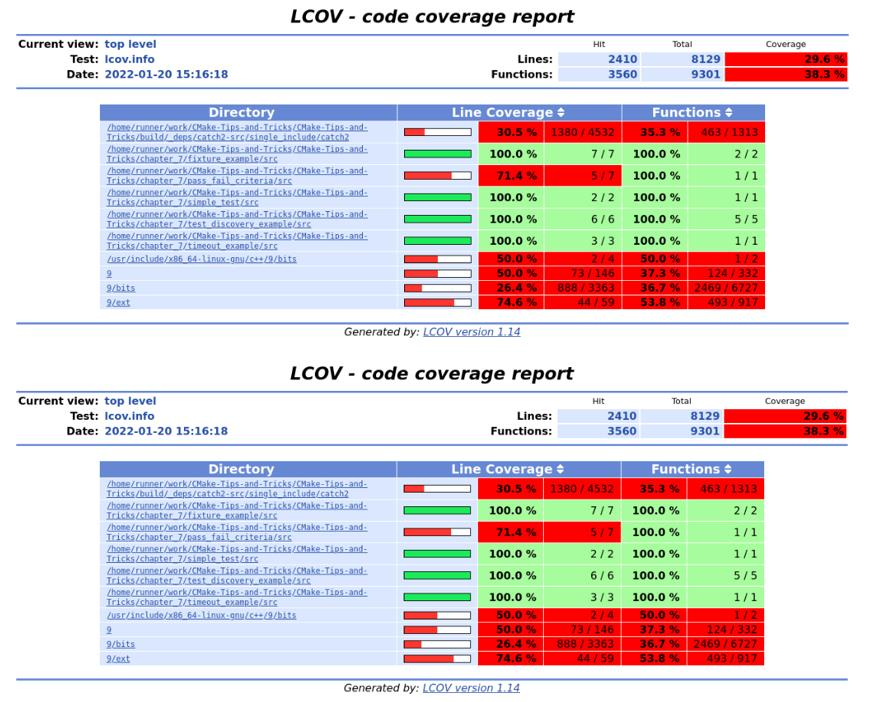
\includegraphics[width=0.8\textwidth]{content/2/chapter7/images/2.jpg}\\
Figure 7.2 – An example coverage report generated with LCOV
\end{center}

Note that these calls will only create coverage reports for the last run. If you want to assemble them into a time series to see whether code coverage goes up or down, there are various CI tools, such as Codecov and Cobertura, available to do this. Such tools can generally parse the output from Gcovr or LCOV and assemble it into fancy graphics showing the coverage trends. The detailed documentation for Gcovr can be found at \url{https://gcovr.com/en/stable/}.

\subsubsubsection{7.3.2\hspace{0.2cm}Creating coverage reports for MSVC}

When building software using Microsoft Visual Studio, the OpenCppCoverage tool is an alternative to Gcov. It works by analyzing the program databases (.pdb) produced by the MSVC compiler rather than by compiling the source with different flags. The command to generate an HTML coverage report for a single executable might look like this:

\begin{tcblisting}{commandshell={}}
OpenCppCoverage.exe --export_type html:coverage.html --
	MyProgram.exe arg1 arg2
\end{tcblisting}

Since this will only generate the coverage report for a single executable, OpenCppCoverage provides the possibility of reading the input from previous rounds and combining them into a report like this:

\begin{tcblisting}{commandshell={}}
OpenCppCoverage.exe --export_type binary:program1.cov --
	program1.exe
OpenCppCoverage.exe --export_type binary:program2.cov --
	program2.exe
OpenCppCoverage.exe --input_coverage=program1.cov --input_
coverage= program2.cov --export_type html:coverage.html
\end{tcblisting}

This will combine the output of the first two runs into a common report. To consume the coverage information, the export\_type option has to be binary.

A common use for coverage reports is to find out how much of the code is covered by the tests defined in a project. In this case, using CTest as the test driver will be convenient. As CTest will run the actual tests as subprocesses, the -{}-cover\_children option has to be passed to OpenCppCoverage. To avoid generating coverage reports for the system libraries used, adding a module and a source filter might be needed. The command could look something like this:

\begin{tcblisting}{commandshell={}}
OpenCppCoverage.exe --cover_children --modules <build_dir> --
	sources <source_dir> -- ctest.exe --build-config Debug
\end{tcblisting}

A slight downside to this approach will be that the coverage report will include a coverage report for CTest itself. The generated HTML report might look like this:

\begin{center}
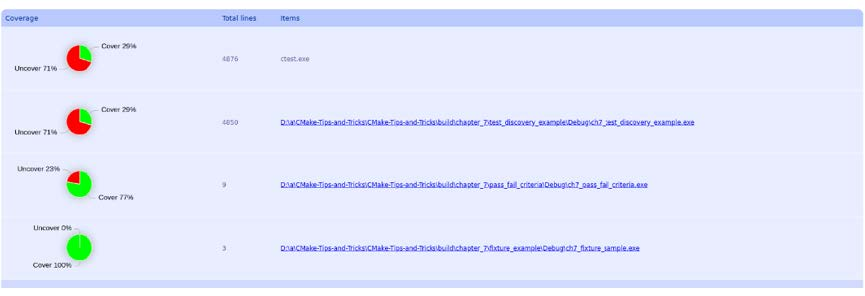
\includegraphics[width=0.8\textwidth]{content/2/chapter7/images/3.jpg}\\
Figure 7.3 – A coverage report generated with OpenCppCoverage
\end{center}

If you are using Visual Studio, an alternative to the command line is to use a plugin for Visual Studio. The plugin can be found on the Visual Studio marketplace: \url{https://marketplace.visualstudio.com/items?itemName=OpenCppCoverage.OpenCppCoveragePlugin}

For the full documentation, consult the GitHub page of OpenCppCoverage:
\url{https://github.com/OpenCppCoverage/OpenCppCoverage}

Knowing how much of your code is covered by the supplied tests is a piece of very valuable information regarding code quality. In fact, in a lot of regulated industries such as medical technology, aviation, or the car industry, providing code coverage reports might be required by the regulatory bodies. However, only knowing how much code is executed is obviously not enough; the quality of the underlying code is of even more importance. Some compilers provide useful tools to detect common errors in your code with the help of so-called sanitizers. In the next section, you will learn how to use and apply sanitizers using CMake.

























